\documentclass[14pt]{extarticle}

\usepackage{fontspec}
\setmainfont{Times New Roman}

% размер полей
\usepackage{geometry}
\geometry{a4paper, top=2cm, bottom=2cm, right=1.5cm, left=3cm}

 %debugging
%\usepackage{showframe}

% полуторный интервал
\usepackage{setspace}
\onehalfspacing

% абзацный отступ
\setlength{\parindent}{1.25cm}

% выравнивание текста по ширине
\sloppy

% списки
\usepackage{calc} % арифметические операции с величинами
\usepackage{enumitem}
\setlist{
    nosep,
    leftmargin=0pt,
    itemindent=\parindent + \labelwidth - \labelsep,
}

% подписи к рисункам и таблицам
\usepackage{caption}
\renewcommand{\figurename}{Рисунок}
\renewcommand{\tablename}{Таблица}
\DeclareCaptionFormat{custom}
{
    \textit{#1#2#3}
}
\DeclareCaptionLabelSeparator{custom}{. }
\captionsetup{
    % хз какой это размер - 12 или нет, но выглядит меньше 14
    font=small,
    format=custom,
    labelsep=custom,
}

% картинки
\usepackage{graphicx}

% колонтитулы
\usepackage{fancyhdr}

% картинки и таблицы находятся именно в том месте текста где помещены (атрибут H)
\usepackage{float}

% таблицы
\usepackage{tabularray}

\graphicspath{ {3.1/models/} }
\usepackage{hyperref}
\usepackage{upgreek}
\begin{document}
\pagestyle{fancy}
\fancyhead{}
% disable header
\renewcommand{\headrulewidth}{0pt}
\singlespacing

\newpage
\begin{center}
    Министерство науки и высшего образования Российской Федерации
    Федеральное государственное автономное образовательное учреждение

    высшего образования

    \guillemotleft МОСКОВСКИЙ ПОЛИТЕХНИЧЕСКИЙ УНИВЕРСИТЕТ\guillemotright

    (МОСКОВСКИЙ ПОЛИТЕХ)
\end{center}
\noindent
\bigbreak
\bigbreak
\bigbreak
\bigbreak
\begin{center}
    \textbf{СВЕДЕНИЯ ИЗ ТЕОРИИ МАРКОВСКИЙ ПРОЦЕССОВ}
    \bigskip
    \bigskip
    \bigskip
    \bigskip
    \bigskip

    Лабораторная работа 3.1

    По курсу \guillemotleft Надёжность информационных систем\guillemotright
    \bigskip

    \bigbreak
    \bigbreak
    \bigbreak
    \bigbreak
\end{center}
\noindent
\bigbreak
\bigbreak
\bigbreak
\bigbreak
\bigbreak
\bigbreak
\bigbreak
\bigbreak
\bigbreak
\bigbreak
\hfill Выполнил

\hfill Дубровских Н.Е.

\hfill Группа 221-361
\bigbreak
\bigbreak
\bigbreak
\hfill Проверил

\hfill Маковей С.О.
\vfill
\begin{center}
    Москва, 2024
\end{center}
\newpage
\onehalfspacing


\begin{center}
    \textbf{Лабораторная работа 3.1}

    \textbf{Общее описание марковского процесса .
Нахождение стационарного коэффициента готовности. Нахождение
нестационарного коэффициента готовности. Оценка вероятности
безотказной работы.}
\end{center}

К \textbf{основным целям} лабораторной работы следует отнести:

\begin{itemize}
    \item формирование у студентов понимания марковских процессов в современных информационных системах и технологиях;
    \item ознакомление студентов с основными понятиями безотказной работы.
\end{itemize}

К \textbf{основным задачам} лабораторной работы следует отнести:

\begin{itemize}
    \item анализа состояния информационных систем и технологий с помощью марковских процессов;
    \item развитие навыков изучения истории и областей применения методов;
    \item развитие навыков классификации характеристик безотказной работы
\end{itemize}
\bigskip

\pagebreak

\begin{center}
\textbf{ОТЧЁТ ПО ВЫПОЛНЕНИЮ}
\end{center}

\textbf{Задача № 1}

В организации «M» действует программно-аппаратное средство
защиты информации (ПАСЗИ), представляющее собой последовательное
соединение элементов в структурной схеме надежности. Заданы
показатели интенсивности отказов по всем элементам. Требуется
определить интенсивность отказов ПАСЗИ, вероятность безотказной
работы и вероятность отказов системы на момент времени t = 80000 ч.
\bigskip

\noindent
\begin{minipage}[H]{\linewidth}
    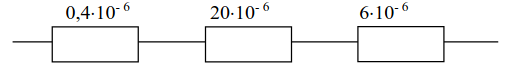
\includegraphics[scale=0.7]{1}
\end{minipage}
\bigskip

\underline{Решение}

\bigskip

\underline{Выводы, вытекающие из решения задачи}

\begin{enumerate}
    \item С увеличением элементов при последовательном соединении
    \item Каково отношение между вероятностью безотказной работы самого надежного элемента и итоговой вероятностью безотказной работы?
\end{enumerate}

\end{document}
